\documentclass[12pt, a4paper]{article}
\usepackage[spanish]{babel}
\usepackage[utf8]{inputenc}
\usepackage{graphicx}
\usepackage{geometry}
\usepackage{fancyhdr}
\usepackage{float}
\usepackage{titling}
\usepackage{hyperref}
\usepackage{url}

% Márgenes
\geometry{a4paper, margin=2.5cm}

% Encabezado y pie de página
\pagestyle{fancy}
\fancyhf{}
\rhead{
\includegraphics[height=1.2cm]{images/logo-usm.png}} % <-- Cambia si usas otro logo
\lhead{Grupo 19\\ Visualización de Datos}
\setlength{\headheight}{20pt}
\setlength{\headsep}{1cm}
\rfoot{Página \thepage}

% Configuración del logo en portada
\pretitle{
  \begin{center}
  \vspace{1cm}
  
\includegraphics[width=0.5\textwidth]{images/logo-usm.png}\\ % <-- Cambia si usas otro logo
  \vspace{1.5cm}
  \LARGE
}
\posttitle{\end{center}}

% Título del informe
\title{Ciberseguridad y Ataques cibernéticos}
\author{Felipe Campaña, Javier Gómez, Matias Elgueta}
\date{\today\\[2cm]}

\begin{document}
\maketitle

% ---------------------------------------------------------------------------------
\vspace*{0.3cm}
\begin{figure}[H]
    \centering
    \begin{minipage}[t]{0.45\linewidth}
    \end{minipage}
    \hfill
    \begin{minipage}[t]{0.45\linewidth}
    \end{minipage}
\end{figure}

% ===================== INTEGRANTE 1 =====================
\section*{Análisis por Integrante}

\subsection*{Integrante 1: Javier Gomez}


\subsubsection*{Gráfico 1: Mapa de puntos categorizados}
\begin{figure}[H]
    \centering
    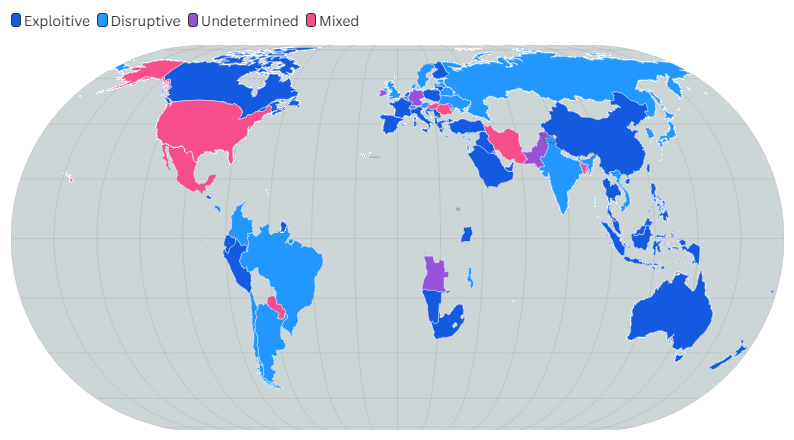
\includegraphics[width=0.9\textwidth]{images/punto_cate.png}
    \caption{Fuente: Elaboración propia con datos}
\end{figure}

\paragraph{Descripción cualitativa del dataset:}

El conjunto de datos contiene información sobre ataques cibernéticos dirigidos a diferentes países. Cada registro describe:
\begin{itemize}
    \item El tipo de actor que realiza el ataque (por ejemplo, \textit{Nation-State}, \textit{Criminal}).
    \item El motivo del ataque (\textit{Sabotage}, \textit{Financial}, etc.).
    \item El tipo de evento (\textit{Exploitive}, \textit{Disruptive}, etc.).
    \item El país objetivo del ataque.
\end{itemize}
Esta información permite clasificar a los países según el tipo de ataque más común que han recibido, representado gráficamente en el mapa mediante distintos colores.

\paragraph{Objetivo de la visualización:}

\begin{itemize}
    \item \textbf{¿Qué pregunta busca responder?} \\
    ¿Qué tipo de ataques cibernéticos predominan en cada país y cómo se distribuyen globalmente?

    \item \textbf{¿A qué público está dirigida?} \\
    A responsables de ciberseguridad, analistas de riesgos, académicos y tomadores de decisiones en políticas públicas.

    \item \textbf{¿Qué acción o decisión podría apoyar?} \\
    Esta visualización puede ayudar a:
    \begin{itemize}
        \item Identificar patrones geográficos de ciberataques.
        \item Establecer prioridades de protección en función del tipo de amenaza.
        \item Fomentar cooperación internacional en ciberseguridad.
    \end{itemize}
\end{itemize}

\paragraph{Conclusiones:}
\begin{itemize}
    \item La mayoría de los países presentan ataques del tipo \textbf{Exploitive}, lo que indica una tendencia a aprovechar vulnerabilidades sin necesariamente causar interrupciones.
    \item Algunos países, como Estados Unidos, muestran una predominancia de ataques \textbf{Disruptive}, que buscan causar interrupciones o daños visibles.
    \item Aparecen categorías \textbf{Mixed} o \textbf{Undetermined} en países donde hay múltiples tipos de ataques o falta de información clara.
    \item Existe una correlación geopolítica: regiones con conflictos o tensiones políticas muestran ataques más agresivos o frecuentes, como en el caso de Ucrania e Irán.
\end{itemize}
\subsubsection*{Anexo: Ataques saboteadores por actores estatales}
\begin{figure}[H]
    \centering
    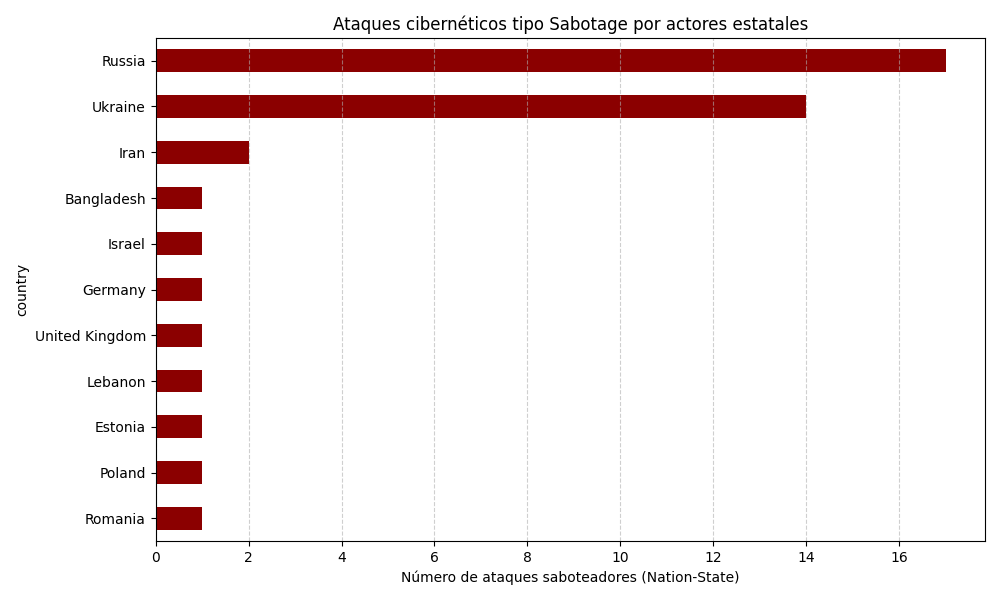
\includegraphics[width=0.8\textwidth]{images/sabotage_state.png}
    \caption{Ataques cibernéticos con motivo de sabotaje realizados por actores estatales. Fuente: Elaboración propia con datos del dataset.}
\end{figure}



\subsubsection*{Gráfico 2: [Nombre del gráfico]}
\begin{figure}[H]
    \
\end{figure}

\textbf{Conclusión:}
\begin{itemize}
    \item ...
\end{itemize}

% ===================== INTEGRANTE 2 =====================
\newpage
\subsection*{Integrante 2: }

% Repite la misma estructura

% ===================== INTEGRANTE 3 =====================
\newpage
\subsection*{Integrante 3: Nombre del estudiante}

% Repite la misma estructura

% ---------------------------------------------------------------------------------
\section{Evidencia de encuesta aplicada}
Aquí puedes insertar una imagen de la base de datos, resumen de resultados o archivo fuente.

\begin{figure}[H]
    \centering
    \caption{Captura de pantalla del archivo Excel con las respuestas de la encuesta}
\end{figure}


\textbf{Repositorio:}  
\label{anexo:repositorio}

Acceso al repositorio en el siguiente link:  
\url{https://github.com/usuario/repositorio.git}

\end{document}
